
\chapter{Jednokrokové algoritmy}
Jednokrokové algoritmy jsou ty, jejichž valuace lze vyjádřit pouze pomocí následující vrstvy potomků. Tedy ohodnocuje kód v závislosti na rozdělení potomků vzhledem k tomuto kódu. V této kapitole porovnáme tři jednokrokové algoritmy, které se liší pouze podle zvoleného prostoru valuací a strategií. Jsou to algoritmy min-max, max entropy a most parts. 

%definujeme následovně. Nechť $G = (V,E)$ je graf [n,k]-Mastermindu. Nechť $\mathcal{F} = \{f_K \mid K \in V \} $ je prostor jednokrokových funkcí, kde $f_K \colon H_{n,k} \to \mathbb{R}$ jsou jednokrokové funkce. Nechť $F$ je funkcionál na $\mathcal{F}$. Potom jednokrokový algoritmus s prostorem funkcí $\mathcal{F}$ a funkcionálem $F$ je definovaný v algoritmu \ref{alg-default}. 



% Nějak popsat to, jak odhadujeme výsledný počet tahů podle tabulky rozdělení - max, entropie, počet částí, očekávaná velikost části v tabulce rozdělení - Irwing, nezmínil jsem.

\section{Min-max}
\begin{definice}[Maximum potomka]
    Nechť $H_{n,k}$ je prostor kódů. Pro $K \subset H_{n,k}$ definujeme funkci maximum potomka jako
    \begin{align*}
        m_K \colon H_{n,k} &\to \mathbb{R} \\
        u &\mapsto \max_{r\in S} |K_{u,r}|.
    \end{align*}
    Prostor všech funkcí $m_K$ označíme $\mathcal{M}$. 
\end{definice}

\begin{definice}[Strategie minimum]
    Nechť $H_{n,k}$ je prostor kódů a $\mathcal{F} = \{f_K\colon H_{n,k} \to \mathbb{R} \mid K \subset H_{n,k}\}$ je prostor valuací. Potom na $\mathcal{F}$ definujeme strategii minimum $L$ jako
    \begin{align*}
        L \colon \mathcal{F} &\to \mathbb{R} \\
        f &\mapsto \min_{u\in H_{n,k}} f(u)
    \end{align*}
\end{definice}

Prvním algoritmem je metoda, kterou navrhl D. Knuth \cite{donald_e__knuth_1977}. Odpovídá algoritmu \ref{alg-default} se vstupním prostorem valuací $\mathcal{M}$ a strategií $L$. Jeho algoritmus tedy vybírá pro další pokus ten kód, který minimalizuje maximální počet kódů v potomcích vzhledem k nějakému kódu. 
%Tedy minimalizuje maximální počet kódů v nějakém stavu, do kterého se hra může dostat po zahrání dalšího kódu.

\begin{definice}[Min-max algoritmus]
    Nechť $n\in \N, k\in \N$, $\mathcal{M}$ je prostor valuací maxima potomků a $M$ je strategie maximum. Min-max algoritmus je definovaný jako funkce 
    \begin{align*}
        \textsc{Solve}[n, k, \mathcal{M}, L] \colon H_{n,k} &\to \mathbb{N} \\
        v & \mapsto \textsc{Solve}[n, k, \mathcal{M}, L](v)
    \end{align*}
    podle předpisu algoritmu \ref{alg-default}.
\end{definice}

Algoritmus Min-max bude v každém kroku (iteraci while cyklu) algoritmu \ref{alg-default} pro množinu kandidátů $K$ vybírat kód z množiny 
%\[U = \{u \in H_{n,k} \mid m_K(u) = L(m_K)\}\] tedy
\[U = \{u \in H_{n,k} \mid \max_{r\in S} |K_{u,r}| = \min_{w \in H_{n,k}} \max_{r\in S} |K_{w,r}| \}\]
Pro [2,2]-Mastermind sestrojíme strom Min-max algoritmu a nastíníme na něm chod Knuthova algoritmu.


\subsubsection{[2,2]-Mastermind}
Prostor kódů [2,2]-Mastermindu je množina $H_{2,2} = \{11,12,21,22\}$. Množina všech ohodnocení je podle tvrzení \ref{tvrzohodnoceni2} rovna $S = \{(0,0), (0,2), (1,0), (2,0)\}$. Na obrázku \ref{fig22prvnitahmnoziny} jsou zobrazeni potomci $H_{2,2}$ vzhledem ke všem kódům a ohodnocením. Pro přehlednost jsou vrcholy uspořádány podle zahraných kódů. Maximální počty prvků ve vrcholech potomků $H_{2,2}$ (hodnoty $m_{H_{2,2}}$) jsou následující. 
\[m_{H_{2,2}} (11) = m_{H_{2,2}} (12) = m_{H_{2,2}} (21) = m_{H_{2,2}} (22) = 2\]
Knuthův algoritmus tedy volí jako první pokus kód $11$. 

\begin{figure}[h!]
    \centering
    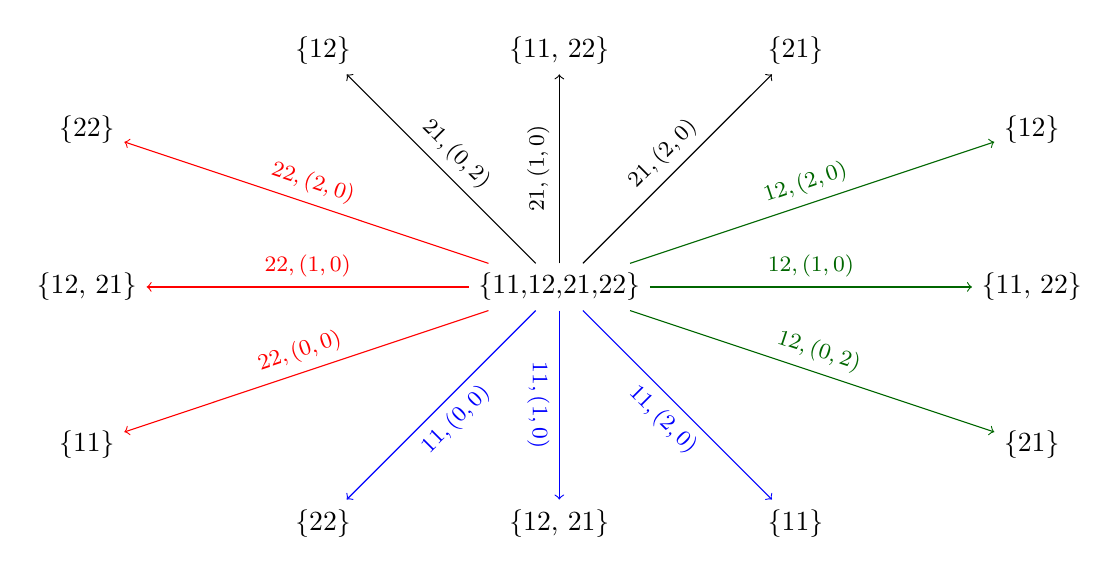
\begin{tikzpicture}
    \node (1) at (0,0) {\{11,12,21,22\}};
    \node (2) at (-3,-3) {\{22\}};
    \draw[->,blue] (1) -- (2) node[pos=0.5, below, sloped] {\footnotesize$11,(0,0)$};
    \node (3) at (0,-3) {\{12, 21\}};
    \draw[->,blue] (1) -- (3) node[pos=0.5, below, sloped] {\footnotesize$11,(1,0)$};
    \node (4) at (3,-3) {\{11\}};
    \draw[->,blue] (1) -- (4) node[pos=0.5, below, sloped] {\footnotesize$11,(2,0)$};
    \node (5) at (6,-2) {\{21\}};
    \draw[->,black!60!green] (1) -- (5) node[pos=0.5, above, sloped] {\footnotesize$12,(0,2)$};
    \node (6) at (6,0) {\{11, 22\}};
    \draw[->,black!60!green] (1) -- (6) node[pos=0.5, above, sloped] {\footnotesize$12,(1,0)$};
    \node (7) at (6,2) {\{12\}};
    \draw[->,black!60!green] (1) -- (7) node[pos=0.5, above, sloped] {\footnotesize$12,(2,0)$};
    \node (8) at (-3,3) {\{12\}};
    \draw[->] (1) -- (8) node[pos=0.5, above, sloped] {\footnotesize$21,(0,2)$};
    \node (9) at (0,3) {\{11, 22\}};
    \draw[->] (1) -- (9) node[pos=0.5, above, sloped] {\footnotesize$21,(1,0)$};
    \node (10) at (3,3) {\{21\}};
    \draw[->] (1) -- (10) node[pos=0.5, above, sloped] {\footnotesize$21,(2,0)$};
    \node (11) at (-6,-2) {\{11\}};
    \draw[->,red] (1) -- (11) node[pos=0.5, above, sloped] {\footnotesize$22,(0,0)$};
    \node (12) at (-6,0) {\{12, 21\}};
    \draw[->,red] (1) -- (12) node[pos=0.5, above, sloped] {\footnotesize$22,(1,0)$};
    \node (13) at (-6,2) {\{22\}};
    \draw[->,red] (1) -- (13) node[pos=0.5, above, sloped] {\footnotesize$22,(2,0)$};
    \end{tikzpicture}
    \caption{Graf všech potomků $H_{2,2}$}
    \label{fig22prvnitahmnoziny}
\end{figure}


Nyní algoritmus volí druhý pokus. Pro $K \neq \emptyset$ a $u \in H_{n,k}$ platí, že $m_K(u) \geq 1$, protože pro $K = \bigsqcup_{r\in S} K_{u,r}$. Proto, když lexikograficky nejnižší kandidát $u$ dosahuje hodnoty $m_K(u) = 1$, algoritmus Min-max ho vždy vybere. Konkrétně to bude platit pro jednoprvkovou množinu kandidátů $\{22\}$. Algoritmus zde jako druhý pokus vybírá jediného zbývajícího kandidáta. 

V případě, že ohodnocení kódu $11$ v prvním pokusu je $(1,0)$, nacházíme se ve stavu $\{12,21\}$. Potomci vrcholu $\{12,21\}$ jsou znázorněni na obrázku \ref{fig22druhytah}. 
\begin{figure}[h!]
    \centering
    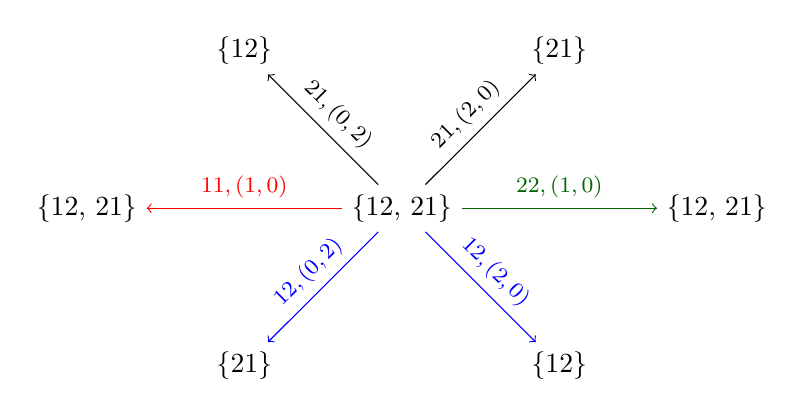
\begin{tikzpicture}
    \node (3) at (0,0) {\{12, 21\}};

    \node (5) at (4,0) {\{12, 21\}};
    \draw[->,black!60!green] (3) -- (5) node[pos=0.5, above,sloped] {\footnotesize$22,(1,0)$};
    
    \node (5) at (-2,-2) {\{21\}};
    \draw[->,blue] (3) -- (5) node[pos=0.5, above,sloped] {\footnotesize$12,(0,2)$};
    \node (6) at (2,-2) {\{12\}};
    \draw[->,blue] (3) -- (6) node[pos=0.5, above,sloped] {\footnotesize$12,(2,0)$};

    \node (7) at (-2,2) {\{12\}};
    \draw[->] (3) -- (7) node[pos=0.5, above,sloped] {\footnotesize$21,(0,2)$};
    \node (8) at (2,2) {\{21\}};
    \draw[->] (3) -- (8) node[pos=0.5, above,sloped] {\footnotesize$21,(2,0)$};

    \node (9) at (-4,0) {\{12, 21\}};
    \draw[->,red] (3) -- (9) node[pos=0.5, above,sloped] {\footnotesize$11,(1,0)$};

    \end{tikzpicture}
    \caption{Výběr druhého tahu}
\label{fig22druhytah}
\end{figure}
Hodnoty valuací jednotlivých kódů jsou následující.
\[m_{\{12,21\}} (11) = m_{\{12,21\}} (22) = 2, \hspace{10px} m_{\{12,21\}} (12) = m_{\{12,21\}} (21) = 1\]
Algoritmus Min-max tedy v tomto stavu vybírá jako druhý pokus kód $12$. 

Na obrázku \ref{fig22minmax} jsou doplněny potomci všech vrcholů vzhledem k zahraným tahům Min-max algoritmu. V případě ohodnocení $(2,0)$ hra končí.
\begin{figure}[h!]
    \centering
    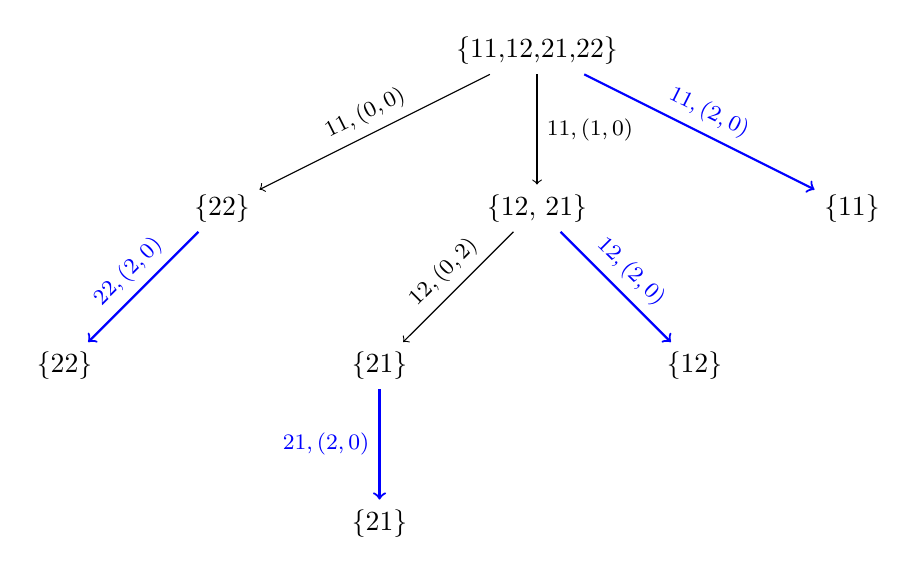
\begin{tikzpicture}
    \node (1) at (0,0) {\{11,12,21,22\}};
    \node (2) at (-4,-2) {\{22\}};
    \draw[->] (1) -- (2) node[pos=0.5, above, sloped] {\footnotesize$11,(0,0)$};
    \node (3) at (0,-2) {\{12, 21\}};
    \draw[->] (1) -- (3) node[pos=0.5, right] {\footnotesize$11,(1,0)$};
    \node (4) at (4,-2) {\{11\}};
    \draw[->, thick, blue] (1) -- (4) node[pos=0.5, above, sloped] {\footnotesize$11,(2,0)$};
    \node (5) at (-2,-4) {\{21\}};
    \draw[->] (3) -- (5) node[pos=0.5, above, sloped] {\footnotesize$12,(0,2)$};
    \node (6) at (2,-4) {\{12\}};
    \draw[->, thick, blue] (3) -- (6) node[pos=0.5, above, sloped] {\footnotesize$12,(2,0)$};
    \node (7) at (-6,-4) {\{22\}};
    \draw[->, thick, blue] (2) -- (7) node[pos=0.5, above, sloped] {\footnotesize$22,(2,0)$};
    \node (8) at (-2,-6) {\{21\}};
    \draw[->, thick, blue] (5) -- (8) node[pos=0.5, left] {\footnotesize$21,(2,0)$};
    \end{tikzpicture}
    \caption{Zahrané tahy min-max algoritmem}
\label{fig22minmax}
\end{figure}
Z tohoto stromu lze vyčíst počet pokusů Min-max algoritmu v případě různých tajných kódů. Je to vzdálenost listu s tímto kódem od kořene ve smyslu počtu hran. Algoritmus Min-max tedy vyhraje [2,2]-Mastermind vždy na maximálně tři tahy. 
    





% Přidat pseudokód algoritmu???

%vysledky Knuthova algoritmu:
% zdroj - Kooi
%expected - 4.476
% maximal - 5
% použít svůj kód a ocitovat

\section{Maximální entropie}
Neuwirth \cite{neuwirth} navrhl algoritmus hrající kódy, které maximalizují entropii velikostí množin potomků vzhledem ke kódu. Nejprve definujeme valuaci a strategii použité v tomto algoritmu. Následně vysvětlíme myšlenku této strategie.

\begin{definice}[Entropie potomků]\label{defentropierozdeleni}
    Nechť $H_{n,k}$ je prostor kódů. Pro $K \subset H_{n,k}$ definujeme valuaci entropie potomků jako funkci
    \begin{align*}
        h_K \colon H_{n,k} &\to \mathbb{R} \\
        u &\mapsto \sum_{r\in S, |K_{u,r}| > 0} \frac{|K_{u,r}|}{|K|}\log_2\left( \frac{|K|}{|K_{u,r}|} \right).
    \end{align*}
    Prostor všech valuací $h_K$ označíme $\mathcal{H}$. 
\end{definice}

\begin{definice}[Strategie maximum]\label{defstrategiemaximum}
    Nechť $H_{n,k}$ je prostor kódů a $\mathcal{F} = \{f_K\colon H_{n,k} \to \mathbb{R} \mid K \subset H_{n,k}\}$ je prostor valuací. Potom na $\mathcal{F}$ definujeme funkcionál maximum $M$ následujícím předpisem.
    \begin{align*}
        M \colon \mathcal{F} &\to \mathbb{R} \\
        f &\mapsto \max_{u\in H_{n,k}} f(u)
    \end{align*}
\end{definice}



\begin{definice}[Algoritmus Max entropy]
    Nechť $n\in \N, k\in \N$, $\mathcal{H}$ je prostor valuací entropie potomků a $M$ je strategie maximum. Algoritmus Max entropy je definovaný jako funkce 
    \begin{align*}
        \textsc{Solve}[n, k, \mathcal{H}, M] \colon H_{n,k} &\to \mathbb{N} \\
        v & \mapsto \textsc{Solve}[n, k, \mathcal{H}, M](v)
    \end{align*}
    podle předpisu algoritmu \ref{alg-default}.
\end{definice}

Níže popíšeme, co si pod pojmem entropie můžeme představit a jaký má význam v [n,k]-Mastermindu.

\begin{definice}[Entropie]\label{defentropie}
  Nechť $A$ je konečná množina, $P \colon A \to [0,1]$ je zobrazení takové, že $\sum_{a \in A} P(a) = 1$. Nechť $supp(P) = \{ a \in A \mid P(a) > 0\}$. Potom entropii zobrazení $P$ definujeme jako 
  \[H(P) = \sum_{a \in supp(P)}P(a)\log_2\left(\frac{1}{P(a)}\right)\]
  Zobrazení $P$ budeme říkat rozdělení, dané hodnotě $P(a)$ pravděpodobnost a množině $[0,1]$ pravděpodobnostní prostor. 
\end{definice}

\begin{pozn}
    Definice \ref{defentropierozdeleni} pro pevný kód $u\in H_{n,k}$ koresponduje s definicí entropie pro množinu všech ohodnocení $A = \{s_1, s_2, \dots, s_m \}$ a zobrazení $P_u\colon A \to [0,1], P_u(s_i) = \frac{|K_{u,r}|}{|K|}$.
\end{pozn}

Co nám ale tato definice říká? Intuici za definicí entropie nastíníme v příkladu \ref{prbinarysearch}, který dává určitý smysl pro výraz $\log_2\left(\frac{1}{P(a)}\right)$ a příkladu \ref{prentropierozdeleni}, který ukazuje příklad entropie na konkrétním rozdělení.

\begin{prikl}[Binární vyhledávání]\label{prbinarysearch}
Představme si, že chceme uhodnout tajné číslo z množiny $\{1,2,\dots,8\}$ pokládáním nějakých ano/ne otázek. Předpokládejme, že každé číslo může být tajným číslem se stejnou pravděpodobností $\frac{1}{8}$. Známým postupem, jak tajné číslo najít je takzvaným půlením intervalu (binární vyhledávání). Vždy se zeptáme, zda je číslo větší nebo menší než číslo v polovině. Nechť tajné číslo je $4$. Binární vyhledávání by mělo následující průběh:

Otázka: "Je číslo větší než $4$?". 
Odpověď: ne

Otázka: "Je číslo větší než $2$?". 
Odpověď: ano

Otázka: "Je číslo větší než $3$?". 
Odpověď: ano

Výsledné číslo je $4$. Počet otázek nutných k určení tajného čísla je $3 = \log_2 8$.
\end{prikl}

\begin{pozn}\label{poznotazkynamnozinu}
Obdobně jako v příkladu \ref{prbinarysearch} lze pro jakoukoliv osmiprvkovou množinu $A$ s rovnoměrnou pravděpodobností vytvořit sadu otázek ano/ne a o každém prvku této množiny určit, zda odpovídá odpovědi ano nebo odpovědi ne. Následně bychom mohli pro určení jakéhokoliv prvku této množiny aplikovat obdobný postup jako v příkladu \ref{prbinarysearch}. Pro vhodnou sadu otázek existuje postup, který každou otázkou sníží prostor zbývajících možností na polovinu. Tím pádem pro určení jakéhokoliv prvku množiny $A$ potřebujeme $\log_2(|A|)$ otázek. V případě, kdy velikost množiny není mocnina $2$ bychom mluvili o $\lceil \log_2 |A| \rceil$, kde $\lceil \cdot \rceil$ značí horní celou část. 
\end{pozn}

\begin{prikl}[m odpovědí]\label{prmodpovedi}
    Ve chvíli, kdybychom nebyli omezeni na ano/ne otázky, ale mohli bychom pokládat otázky na které bychom dostali $m$ odpovědí, mohli bychom aplikovat obdobný postup jako v příkladu \ref{prbinarysearch} s binárním vyhledáváním. Tentokrát bychom ale mohli po každé otázce snížil prostor zbývajících možností $m$-krát. Dobrali bychom se k výsledku, že očekávaný počet otázek k určení prvku z množiny $A$ by byl $\log_m |A|$.
\end{prikl}

\begin{prikl}\label{prentropierozdeleni}
Nechť $A = \{ \text{a, b, c, d}\}$ a $P$ je zadaná následovně: 
\[P(a) = \frac{1}{8}, P(b) = \frac{1}{8}, P(c) = \frac{1}{4}, P(d) = \frac{1}{2}\]
Nyní si představme pravděpodobnostní prostor jako čtverec na obrázku \ref{prprostor}, kde pravděpodobnost prvku je velikost plochy. Výraz $\frac{1}{P(a)}$ říká, kolik prvků $A$ s touto pravděpodobností by se "vešlo" do pravděpodobnostního prostoru jako na obrázku. Například dílek c by se "vešel" do pravděpodobnostního prostoru čtyřikrát.
Hodnota $\log_2\left(\frac{1}{P(c)}\right)$ lze interpretovat jako počet otázek ano/ne, který potřebujeme k jednoznačnému určení prvku c v případě, kdyby byl pravděpodobnostní prostor rozdělen rovnoměrně. Tento postup byl popsán 
%v příkladu \ref{prbinarysearch} a 
v poznámce \ref{poznotazkynamnozinu}.
Entropie tohoto rozdělení by v tomto případě byla 
\[H(P) = \frac{1}{8}\log_2 (8) + \frac{1}{8}\log_2 (8) + \frac{1}{4}\log_2 (4) + \frac{1}{2}\log_2 (2) = \frac{3}{8} + \frac{3}{8} + \frac{2}{4} + \frac{1}{2} = \frac{7}{4}\]
a můžeme ji interpretovat jako očekávaný počet otázek, který potřebujeme k jednoznačnému určení prvku z množiny $A$. 


\begin{figure}
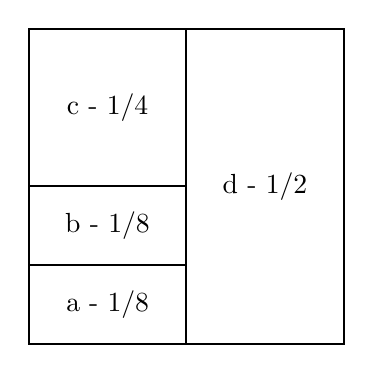
\begin{tikzpicture}
    \draw[black, thick] (0,0) rectangle (4,4);
    \begin{scope}
        \node (1) at (1,0.5) {a - 1/8};
        \node (2) at (1,1.5) {b - 1/8};
        \node (3) at (1,3) {c - 1/4};
        \node (4) at (3,2) {d - 1/2};
    \end{scope}
    \draw[black, thick] (2,0) -- (2,4);
    \draw[black, thick] (0,2) -- (2,2);
    \draw[black, thick] (0,1) -- (2,1);

    
\end{tikzpicture}
\caption{Pravděpodobnostní prostor}
\label{prprostor}
\end{figure}

\end{prikl}

\subsubsection{Entropie a Mastermind}
Nyní vysvětlíme, jakým způsobem aplikujeme výpočet entropie na strategii pro řešení [n,k]-Mastermindu. Otázky v předchozích příkladech nahradíme zahranými pokusy. Jako odpovědi budou sloužit ohodnocení pokusů. Nechť $K$ je aktuální množina kandidátů. Pro $K$ můžeme ve smyslu příkladu \ref{prmodpovedi} definovat nějakou abstraktní hodnotu počtu pokusů potřebných k určení jakéhokoliv prvku  $v \in K$ jako $\log_{|S|}(|K|)$. Na každý pokus můžeme totiž dostat maximálně $|S|$ možných ohodnocení. 

Nechť $u \in H_{n,k}$ je kód a $S$ je množina všech možných ohodnocení kódů v $H_{n,k}$. Potom $\{K_{u,r} \mid r\in S\}$ jsou potomci $K$ vzhledem ke kódu $u$ a $\log_{|S|}(|K_{u,r}|)$ je očekávaný počet pokusů k určení jakéhokoliv prvku $v \in K_{u,r}$. Pomocí těchto hodnot lze vytvořit odhad na počet pokusů potřebných k určení jakéhokoliv kódu $v \in K$ po zahrání kódu $u$ jako 
\begin{align}\label{rceocekavanypocetpokusu}
    G = \sum_{i=1}^n \frac{|K_{u,r}|}{|K|}\log_{|S|}|K_{u,r}|.
\end{align}



%Pro každé $K_i, i \in \{1, 2, \dots, m\}$ můžeme ve smyslu poznámky \ref{poznotazkynamnozinu} definovat nějakou abstraktní hodnotu počtu otázek ano/ne potřebných k určení jakéhokoliv prvku  $x \in K_i$ jako $\log_2(|K_i|)$. Potom obdobně jako v příkladu \ref{prentropierozdeleni} můžeme určit očekávaný počet otázek jako
%\[G = \sum_{i =1}^n \frac{|K_i|}{|K|}\log_2|K_i| \]
Tato hodnota bude naším stavebním kamenem pro strategii za užití entropie. Protože cílem [n,k]-Mastermindu je najít tajný kód v co nejmenším počtu pokusů, chceme hodnotu $G$ minimalizovat. 

%\[ u = \arg\min_{w \in H_{4,6}} \sum_{i =1}^n \frac{|K_i|}{|K|}\log_2|K_i|\]

\begin{veta}[Ekvivalence maximalizace entropie] \label{vetaekvivalencemaxentropy}
    Uvažujme [n,k]-Mastermind s tajným kódem $v\in H_{n,k}$. Označme $K$ množinu kandidátů. Potom 
    \begin{align}\label{rceproentropii}
        \sum_{r\in S} \frac{|K_{u,r}|}{|K|}\log_{|S|}|K_{u,r}| = \min_{w \in H_{n,k}} \sum_{r\in S} \frac{|K_{w,r}|}{|K|}\log_{|S|}|K_{w,r}|
    \end{align}
    právě tehdy, když 
    \[h_K(u) = \max_{w \in H_{n,k}} h_K(w) \]
    
\end{veta}
\begin{dukaz} Využíváme toho, že pro $x \in \mathbb{R}$ a konečnou množinu reálných čísel $A$ platí vztahy.
\[z \cdot \min\{a \mid a \in A\} = \min\{z\cdot a \mid a \in A\} \textrm{ pro } z \geq 0\]
a 
\[z \cdot \min \{a \mid a \in A\} = \max\{z\cdot a \mid a \in A\}\textrm{ pro } z < 0.\]
Navíc platí $\log_{|S|} |K_{u,r}| = \frac{\log |K_{u,r}|}{\log |S|}$, a tedy
    \[\log_{2} |K_{u,r}| = \log_{|S|} |K_{u,r}| \cdot \frac{\log |S|}{\log 2}\]
Po přenásobení rovnosti \ref{rceproentropii} konstantou $\frac{\log|S|}{\log2}$ dostáváme
\[\sum_{r\in S} \frac{|K_{u,r}|}{|K|}\log_{2}|K_{u,r}| = \min_{w \in H_{n,k}} \sum_{r\in S} \frac{|K_{w,r}|}{|K|}\log_{2}|K_{u,r}|\]
Tuto rovnici přenásobíme konstantou $(-1)$ a převrátíme argument logaritmu.
\[\sum_{r\in S} \frac{|K_{u,r}|}{|K|}\log_{2}\frac{1}{|K_{u,r}|} = \max_{w \in H_{n,k}} \sum_{r\in S} \frac{|K_{w,r}|}{|K|}\log_{2}\frac{1}{|K_{u,r}|}\]
Následně k oběma stranám přičteme hodnotu $\log_2|K|$.

\[\sum_{r\in S} \frac{|K_{u,r}|}{|K|}\log_{2}\frac{|K|}{|K_{u,r}|} = \max_{w \in H_{n,k}} \sum_{r\in S} \frac{|K_{w,r}|}{|K|}\log_{2}\frac{|K|}{|K_{w,r}|}\]
Využili jsme toho, že $\sum_{i=1}^n \frac{|K^u_i|}{|K|} = 1$ a součtového vzorce pro logaritmus. Z definice $h_K$ plyne 
\[h_K(u) = \max_{w \in H_{n,k}}  h_K(w) .\]
Všechny úpravy byly ekvivalentní, a tedy jsme hotovi.
\end{dukaz}

Dokázali jsme tedy, že kódy, které minimalizují očekávaný počet pokusů ve smyslu rovnice \ref{rceocekavanypocetpokusu} jsou právě ty kódy, které maximalizují entropii rozdělení z definice \ref{defentropierozdeleni}. To je myšlenka algoritmu Max entropy. 





% Funkce $\log_2(x)$ je rostoucí, a proto tato hodnota určitým způsobem koresponduje s 
% možná by šlo napsat větu, že tabulka rozdělení plyne pouze z kandidátů a dalšího kódu. 



% Tato strategie lze přeformulovat jako minimalizace (přes všechny kódy) očekávaného počtu otázek ano/ne, které jsou nutné pro určení tajného kódu po zahrání dalšího tahu.

% Nechť máme množinu $K$, definujeme počet otázek ano/ne potřebných k určení jakéhokoli prvku $s \in K$ jako $\log_2(|K|)$. Všimněme si, že tato definice koresponduje s příkladem \ref{prbinarysearch}, v případě, když každému prvku množiny 
%V našem případě ale kvůli pravidlům hry nelze jednoduše definovat očekávaný počet ano/ne otázek na určení nějakého kódu, protože se nemůžeme cíleně ptát: "je na i-té pozici k-tá barva?". Navíc nedostáváme odpovědi ano/ne.


% Lze to tedy formulovat i tak, že tah maximalizuje střední hodnotu informačního obsahu po ohodnocení tahu. Informační obsah představuje $-log(\frac{|K_i|}{|K|})$, kde |K| je počet kandidátů před zahráním tahu. Tedy je to nějaká hodnota informace vztažená na počet kandidátů. Algoritmus tedy hledá 


\section{Počet potomků}
Další strategie, kterou navrhl Barteld Kooi \cite{kooi} je volba kódu, který maximalizuje počet ohodnocení, které jako další pokus může dostat. Formálně tento počet definujeme jako počet neprázdných potomků.
\begin{definice}[Počet potomků]
    Nechť $H_{n,k}$ je prostor kódů. Pro $K \subset H_{n,k}$ definujeme valuaci počet potomků jako
    \begin{align*}
        c_K \colon H_{n,k} &\to \mathbb{R} \\
        u &\mapsto |\{r \mid K_{u,r} \neq \emptyset\}|
    \end{align*}
    Prostor všech valuací $c_K, \hspace{3px} K \subset H_{n,k}$ označíme $\mathcal{C}$. 
\end{definice}

\begin{definice}[Algoritmus Most parts]
    % Nechť $n\in \N, k\in \N$. Algoritmus s počtem potomků je pro vstupní tajný kód $v\in H_{n,k}$ definovaný jako $\text{\textsc{SolveMastermind}} (n,k,s_v, \mathcal{C}, M)$. Zde $s_v$ značí zobrazení z definice \ref{defohodnocenivzhledem} a $M$ je funkcionál maximum.

     Nechť $n\in \N, k\in \N$, $\mathcal{C}$ je prostor valuací počtu potomků a $M$ je strategie maximum. Algoritmus Most parts je definovaný jako funkce 
     \begin{align*}
         \textsc{Solve}[n, k, \mathcal{C}, M] \colon H_{n,k} &\to \mathbb{N} \\
         v & \mapsto \textsc{Solve}[n, k, \mathcal{C}, M](v)
     \end{align*}
     podle předpisu algoritmu \ref{alg-default}.
\end{definice}
Tato strategie je motivována následujícími příklady, které Kooi popisuje ve svém článku. 

\begin{prikl}\label{prdvecasti}
    Uvažujme klasický balíček $52$ karet. Naším úkolem je uhodnout tajnou kartu s tím, že každá karta může být tou tajnou se stejnou pravděpodobností. Předtím se ale můžeme zeptat na jednu ano/ne otázku, kterou snížíme počet zbývajících možností. Jak máme tuto otázku zvolit? 
    Pokud bychom se zeptali, zda je karta srdcová, pravděpodobnost, že kartu po této otázce uhodneme je 
    \[\frac{13}{52} \cdot \frac{1}{13} + \frac{39}{52} \cdot \frac{1}{39} = \frac{2}{52}.\]
    Pokud se zeptáme, zda tajnou kartou je piková sedmička, pravděpodobnost, že kartu po této otázce uhodneme je 
     \[\frac{1}{52} \cdot 1 + \frac{51}{52} \cdot \frac{1}{52} = \frac{2}{52}.\] 
    Nezáleželo tedy, na jak velké množiny nám otázka balíček karet rozdělila. 
\end{prikl}\textbf{}

\begin{prikl}
    Nechť nyní můžeme dostat $k$ různých odpovědí na položenou otázku. Definujeme $K_i$ množinu karet vyhovujících odpovědi $i$. Předpokládáme, že žádná karta nemůže vyhovovat dvěma odpovědím na položenou otázku. Pravděpodobnost, že tajnou kartu uhádneme po této otázce je 
\[\sum_{i = 1}^k \frac{|K_i|}{52} \cdot \frac{1}{|K_i|} = \frac{k}{52}.\]
\end{prikl}


Z těchto dvou příkladů tedy plyne, že nezáleží na velikostech množin, na které otázka rozdělí karty, ale záleží na jejich počtu. Obdobný postup lze aplikovat na hru [n,k]-Mastermind. Jako v případě entropie uvažujeme místo otázek a odpovědí pokusy a jejich ohodnocení. Množiny, na které se množina kandidátů na tajný kód rozdělí jsou neprázdní potomci vzhledem k zahranému kódu. 

%V případě hry [n,k]-Mastermind porovnáváme pravděpodobnosti uhodnutí tajného kódu po daném pokusu. Hledáme tedy kód, který maximalizuje počet možných ohodnocení. Tabulka~\ref{tab02} ukazuje počty možných ohodnocení prvních tahů. Tato strategie by vybrala kód 1123, nebo 1234. 

%Kooi ukázal, že za použití této strategie lze dosáhnout očekávaného počtu pokusů $4.373$. Podrobněji jsou výsledky popsány v následující kapitole.

%V závěru Kooi diskutuje nad možnými zlepšeními/atd - šlo by zmínit








%\subsection{Očekávaný počet}